\documentclass[11pt]{article}
\usepackage[a4paper,margin=0.92in]{geometry}
\usepackage{amsmath,amssymb,booktabs,array,graphicx,float}
\usepackage{enumitem}
\usepackage{microtype}
\usepackage[hidelinks]{hyperref}
\setlength{\parindent}{1.5em}
\setlength{\parskip}{0pt}
\renewcommand{\arraystretch}{1.10}
\setcounter{tocdepth}{1}

\title{The Informax Decoupler in ScaPre:\
Effects of Channel Weighting on Concept Removal and Preservation}
\author{Tse-An Li\\
Department of Applied Mathematics, National Yang Ming Chiao Tung University\\
Advisors: Te-Sheng Lin and Jia-Wei Liao}
\date{September 2026}

\begin{document}
\maketitle

\begin{abstract}
ScaPre's Informax Decoupler assigns channel-specific weights from the mutual information (MI) between median-binarized activations and target or neutral labels. This report analyzes the resolution of that estimator and tests whether the channel weights used by the released repository improve image-level results. With the repository default of $5+5$ target and empty-string samples, $98.51\%$ of observations reach the maximum MI. The fraction remains $97.17\%$ with $50+50$ samples. Maximizing MI over target concepts increases the saturation: in the measured ten-target data, every aggregated channel reaches maximum MI from four targets onward, which gives $B=I$ under the paper's normalization. The repository uses a different transform and solver that retain small differences among channels. Across five seeds, replacing its final weight vector with a per-matrix constant, a shuffled vector, or a vector of ones causes little change in the image metrics. The choice of negative reference affects the removal--preservation trade-off, but the best-performing reference uses retain concepts from the evaluation and is suitable only as a diagnostic. Two squared-cosine alternatives also fail to give a consistent improvement. These results do not assess every use of Informax in ScaPre. They show that binary MI offers little channel resolution under the tested protocol and that the benefit of the final channel assignment is not visible in these experiments.
\end{abstract}

\begingroup
\small
\tableofcontents
\endgroup
\newpage

\section{Introduction}
ScaPre is a closed-form method for removing multiple concepts from a text-to-image diffusion model while preserving related and unrelated content \cite{scapre}. Its Informax Decoupler is meant to identify concept-relevant output channels and give those channels different weights during editing. That description depends on two things: the MI estimator must distinguish channels, and the resulting weights must matter when they are assigned to particular channel identities.

This project examines four questions:
\begin{enumerate}[label=\arabic*.]
    \item How many distinct values can the median-binarized MI estimator produce, and why does it saturate under the official empty-string reference?
    \item What happens after MI is aggregated across several target concepts?
    \item Do the final repository channel weights outperform simple controls that remove or scramble channel identity?
    \item Can a continuous directional score avoid the saturation without damaging concept removal?
\end{enumerate}

The mathematical analysis identifies where the estimator can lose resolution. The image experiments then test the final channel assignment while leaving the earlier Informax-weighted accumulation and the rest of ScaPre unchanged.

\section{Paper Formulation and Released Implementation}
\label{sec:paper_repo}
\subsection{Informax in the paper}
For output channel $i$, ScaPre forms noisy target and neutral samples, maps them through the current projection row, and binarizes the activation at a channel-wise threshold. Let $Z_i\in\{0,1\}$ be the binarized activation and $Y\in\{0,1\}$ the neutral/target label. The paper defines
\begin{equation}
    MI_i=\sum_{z,y}p_i(z,y)
    \log\frac{p_i(z,y)}{p_i(z)p_i(y)}.
    \label{eq:mi_general}
\end{equation}
For several target concepts, it then takes
\begin{equation}
    MI_i=\max_k MI_i^{(k)},
    \qquad
    \alpha_i=\frac{MI_i}{\max_j MI_j},
    \qquad
    B=\operatorname{diag}(\alpha_1,\ldots,\alpha_d).
    \label{eq:paper_alpha}
\end{equation}
The paper's quadratic objective leads to the Sylvester equation
\begin{equation}
    BW+WA=V^{*}C_E^{\top}.
    \label{eq:paper_sylvester}
\end{equation}
Because $B$ is diagonal, its row-wise form is
\begin{equation}
    w_i(A+\alpha_i I)=m_i,
    \label{eq:paper_row}
\end{equation}
where $w_i$ and $m_i$ are the corresponding rows. Under this formulation, differences among the $\alpha_i$ are exactly what give output channels different penalties.

\subsection{Weighting in the released repository}
The released repository \cite{scaprecode} does not use the direct normalization in Eq.~\eqref{eq:paper_alpha}. For each target concept, projection, and edited matrix, it applies
\begin{equation}
\begin{aligned}
&\text{target/neutral vectors}
\rightarrow \text{noisy pseudo-samples}
\rightarrow W_{\mathrm{old}}s
\rightarrow \text{median threshold}
\rightarrow MI\\
&\hspace{3.0cm}\rightarrow z\text{-score}
\rightarrow \operatorname{sigmoid}(z/0.7)^8.
\end{aligned}
\end{equation}
The final repository weight is
\begin{equation}
    \alpha_i=\max_k
    \left[
    \operatorname{sigmoid}\left(
    \frac{MI_i^{(k)}-\mu^{(k)}}{0.7(s^{(k)}+\varepsilon)}
    \right)
    \right]^8.
    \label{eq:repo_alpha}
\end{equation}
This nonlinear transform preserves small differences even when most raw MI values are tied near their maximum.

Informax is used twice in the executed edit. A fresh per-concept weight first multiplies the row contribution during UCE accumulation. A second set of weights is aggregated across targets and enters the final row-wise solve. The controls in Sec.~\ref{sec:alpha_controls} modify only this second set; the earlier use remains active.

\subsection{Solver used by the released repository}
The released code does not execute Eq.~\eqref{eq:paper_sylvester} directly. For each row it constructs
\begin{equation}
    M_i=G_{\mathrm{base}}+s_e\alpha_i\Pi_C,
    \qquad
    b_i=(\lambda+\mu)w_{\mathrm{old},i}+v_i,
    \qquad
    M_i w_i^{\top}=b_i^{\top},
    \label{eq:repo_solver}
\end{equation}
followed by the Bures proximal step, where $s_e$ is the erase scale and $\Pi_C$ is an input-side concept-subspace projector. The repository weight therefore scales one input-side term in a hybrid row system; it is not simply the output-side $B$ from the paper equation.

This distinction determines how the two results should be interpreted. The finding that the paper's aggregation gives $B=I$ follows from Eqs.~\eqref{eq:paper_alpha}--\eqref{eq:paper_sylvester}. The \texttt{identity\_B} experiment instead sets every final repository weight $\alpha_i$ to one inside Eq.~\eqref{eq:repo_solver}; it does not reproduce the complete solver described in the paper.

\section{Experimental Protocol}
\label{sec:protocol}
All image-level comparisons use the same project-established reconstruction of ImageNet-Confuse5. It is derived from public ScaPre assets, but the exact generation assets behind the paper's Table~7 were not released. Results are therefore interpreted within this protocol, not as an exact reproduction of the paper table.

\begin{table}[H]
\centering
\caption{Fixed generation, editing, and evaluation settings.}
\begin{tabular}{>{\raggedright\arraybackslash}p{0.28\textwidth}>{\raggedright\arraybackslash}p{0.62\textwidth}}
\toprule
Item & Setting \\
\midrule
Base model & Stable Diffusion v1.5, snapshot \texttt{451f4fe16113bff5a5d2269ed5ad43b0592e9a14} \\
Concepts & 10 targets and 15 similar retain concepts in five groups \\
Edit seeds & 20260820, 20260821, 20260822, 20260823, 20260824 \\
Images & 120 per concept; 3000 per seed and variant \\
Prompt & \texttt{an image of a \{concept\}} \\
Generation & PNDM scheduler, 50 steps, CFG 7.5, $512\times512$, float16 \\
Evaluation & ImageNet ResNet-50 top-1 prediction; lowercase substring label match \\
Edit settings & erase scale 2, power $p=8$, one Bures iteration, ASED enabled, single-space target replacement \\
Informax settings & 5 positive and 5 negative samples, noise $\sigma=0.01$, temperature 0.7 \\
Entropy settings & 30 samples, 20 bins, $T_\sigma=p_\sigma=1$ \\
\bottomrule
\end{tabular}
\end{table}

The three image metrics are:
\begin{itemize}
    \item \textbf{Unlearn Accuracy} $U$ (lower is better): residual target accuracy;
    \item \textbf{Preserve Accuracy} $P$ (higher is better): accuracy on the similar retain concepts;
    \item \textbf{Overall Accuracy} $O$ (higher is better):
    \begin{equation}
        O=\frac{2(100-U)P}{(100-U)+P}.
        \label{eq:overall}
    \end{equation}
\end{itemize}
Unless stated otherwise, a reported delta is treatment minus official. Thus a negative $\Delta U$ and positive $\Delta P,\Delta O$ are favorable. Generation keys, row counts, evaluator fingerprints, and official score hashes were checked across the controlled runs.

\section{Why the Binary MI Has Few Values}
\label{sec:mi_math}
\subsection{The contingency table}
Consider one channel, with $n$ target and $n$ neutral pseudo-samples. The channel-wise median divides the $2n$ activations into an upper and lower half when there are no exact threshold ties. Let $K$ be the number of target samples in the upper half. Balanced labels and the median split force the whole table to be
\begin{equation}
\begin{array}{c|cc}
 & Y=1\text{ (target)} & Y=0\text{ (neutral)} \\ \hline
Z=1 & K & n-K \\
Z=0 & n-K & K
\end{array}.
\label{eq:tableK}
\end{equation}
Thus the MI is determined by one integer, $K$.

\subsection{Explicit simplification and symmetry}
Ignoring the implementation's tiny symmetric pseudocount for readability, each row and column marginal equals $1/2$. Substituting Eq.~\eqref{eq:tableK} into Eq.~\eqref{eq:mi_general} gives
\begin{align}
MI(K)
&=2\frac{K}{2n}
\log\frac{K/(2n)}{(1/2)(1/2)}
+2\frac{n-K}{2n}
\log\frac{(n-K)/(2n)}{(1/2)(1/2)} \notag\\
&=\frac{K}{n}\log\frac{2K}{n}
+\frac{n-K}{n}\log\frac{2(n-K)}{n} \notag\\
&=MI(n-K),
\label{eq:mi_closed}
\end{align}
with the usual convention $0\log0=0$. The last equality is visible directly: replacing $K$ by $n-K$ only swaps the two terms.

Therefore only
\begin{equation}
    \left\lfloor\frac n2\right\rfloor+1
\end{equation}
different MI values are possible in the no-tie case. At $n=5$, the three values are approximately $0.0201$, $0.1927$, and $0.6931=\ln2$. The smallest is not zero because odd $n$ cannot divide each label evenly between the two activation states. The repository's symmetric pseudocount changes these values only negligibly. Exact threshold ties can create extra count patterns, but they do not change the main conclusion: binarization gives a coarse score.

\section{Empirical Saturation}
\label{sec:saturation}
\subsection{Increasing the sample size}
To check whether the observed saturation is only a consequence of using $5+5$ samples, a fixed pool of 50 target and 50 empty-string samples was generated for each seed. Smaller settings use nested prefixes of the same pool.

\begin{table}[H]
\centering
\caption{Effect of pseudo-sample count under the official empty-string reference.}
\begin{tabular}{rrrrr}
\toprule
$n+n$ & Mean MI & Fraction at $\ln2$ & Repo $\alpha$ mean & Repo $\alpha$ p99 \\
\midrule
$5+5$ & 0.684657 & 98.5094\% & 0.007434 & 0.009455 \\
$10+10$ & 0.683318 & 98.0369\% & 0.007984 & 0.010383 \\
$20+20$ & 0.682585 & 97.6294\% & 0.008302 & 0.010843 \\
$50+50$ & 0.682101 & 97.1658\% & 0.008509 & 0.011115 \\
\bottomrule
\end{tabular}
\end{table}

\begin{figure}[H]
\centering
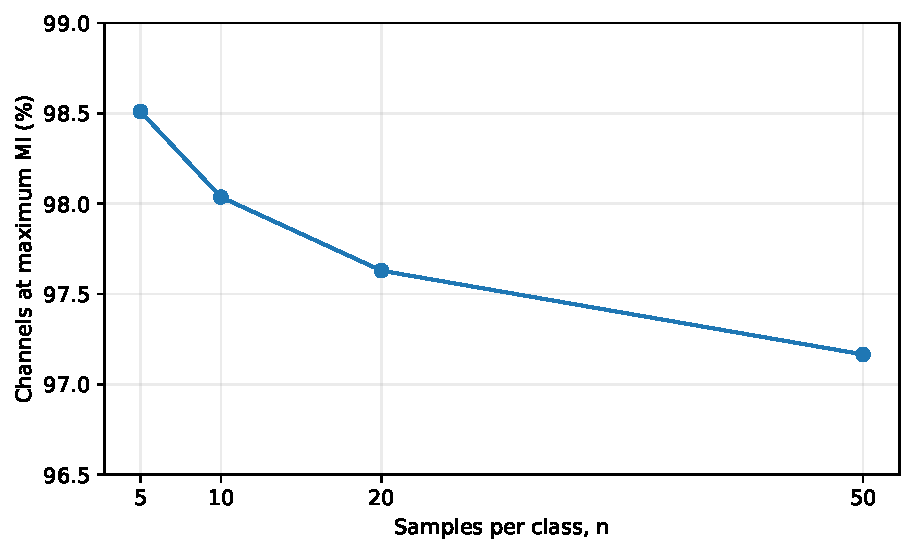
\includegraphics[width=0.68\textwidth]{figures/sample_size_saturation.pdf}
\caption{Maximum-MI fraction as the target and neutral sample counts increase.}
\end{figure}

A tenfold increase in sample count lowers the maximum-MI fraction by only $1.34$ percentage points. Among observations at maximum MI for $n=5$, $98.64\%$ remain there at $n=50$. The coarse estimator contributes to the limited resolution, but sample count is not the main explanation: target text and empty text are already separated almost perfectly for most measured channels.

\subsection{Maximum over target concepts}
For $m$ target concepts, the paper uses
\begin{equation}
    MI_i^{(m)}=\max_{1\leq k\leq m}MI_i^{(k)}.
\end{equation}
The maximum can only increase as $m$ grows. Since one concept already gives maximum MI for most observations, adding concepts gives every channel more chances to reach the maximum.

All $1023$ non-empty subsets of the ten measured targets were enumerated. The values below are averages over subsets of the same size. Four concepts suffice in these measurements, but this is an empirical result rather than a general theorem.

\begin{table}[H]
\centering
\caption{Maximum over $m$ target concepts as defined in the paper.}
\begin{tabular}{rrrr}
\toprule
$m$ & Fraction at max MI & Fraction $\alpha=1$ & Mean $\alpha$ \\
\midrule
1 & 98.5094\% & 98.5094\% & 0.987751 \\
2 & 99.9739\% & 99.9739\% & 0.999802 \\
3 & 99.9997\% & 99.9997\% & 0.999998 \\
4 & 100\% & 100\% & 1.000000 \\
10 & 100\% & 100\% & 1.000000 \\
\bottomrule
\end{tabular}
\end{table}

\begin{figure}[H]
\centering
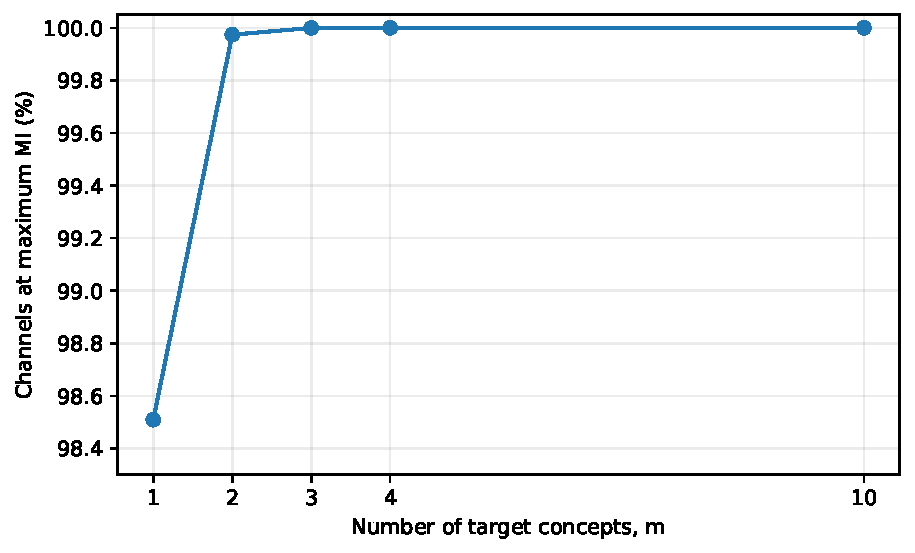
\includegraphics[width=0.68\textwidth]{figures/paper_concept_max.pdf}
\caption{The concept-wise maximum amplifies single-concept saturation.}
\end{figure}

From four targets onward, every measured channel has aggregated $MI_i=\ln2$. Equation~\eqref{eq:paper_alpha} then gives
\begin{equation}
    \alpha_i=\frac{\ln2}{\ln2}=1
    \quad\text{for all }i,
    \qquad B=I.
\end{equation}
The paper's output-side term becomes
\begin{equation}
    \operatorname{tr}(W^{\top}BW)
    =\operatorname{tr}(W^{\top}W)
    =\|W\|_F^2,
\end{equation}
so it no longer distinguishes output channels.

The repository transform in Eq.~\eqref{eq:repo_alpha} prevents the weights from becoming exactly one. Its mean final $\alpha$ changes from $0.007434$ at one target to $0.008642$ at ten targets.

\begin{figure}[H]
\centering
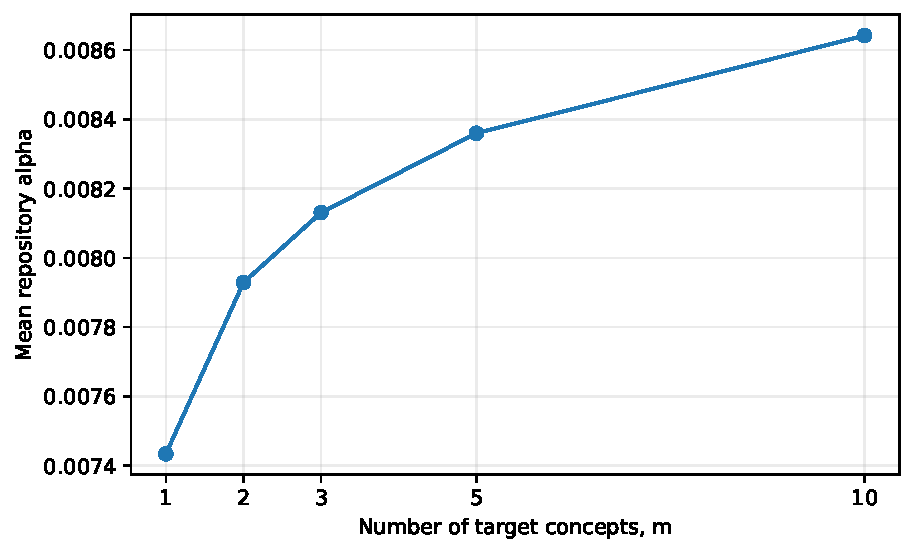
\includegraphics[width=0.68\textwidth]{figures/repo_alpha_concept_count.pdf}
\caption{Mean repository final $\alpha$ as the number of targets increases.}
\end{figure}

The remaining question is whether these small differences are useful because they are attached to the right channel identities.

\section{Controls for the Final Channel Weights}
\label{sec:alpha_controls}
\subsection{Interventions}
The control runner replaces only the final aggregate vector after the official MI $\rightarrow$ z-score $\rightarrow$ sigmoid/power $\rightarrow$ concept-max path and before Eq.~\eqref{eq:repo_solver}. The production editor itself remains unchanged.

\begin{table}[H]
\centering
\caption{Meaning of the four final-weight variants.}
\begin{tabular}{>{\raggedright\arraybackslash}p{0.22\textwidth}p{0.67\textwidth}}
\toprule
Variant & Intervention \\
\midrule
official & Keep the repository final $\alpha$ vector. \\
constant\_mean & Replace every entry in a matrix by that matrix's mean $\bar\alpha$. This removes channel differences while roughly preserving the usual scale. \\
shuffled & Keep the exact per-matrix multiset of values but assign it to channels through a fixed preregistered permutation. This tests channel identity. \\
identity\_B & Set every final $\alpha_i$ to one. This tests unit weights and also changes the scale. \\
\bottomrule
\end{tabular}
\end{table}

Raw MI, per-concept weights, thresholds, random tensors, UCE inputs, prompts, generation seeds, sampler, and evaluator are held fixed. In particular, \texttt{constant\_mean} does not remove Informax from the whole editor: the earlier per-concept Informax weighting remains.

\subsection{Image-level results}
\begin{table}[H]
\centering
\caption{Five-seed metrics. Each cell is Unlearn / Preserve / Overall (\%).}
\resizebox{\textwidth}{!}{%
\begin{tabular}{lcccc}
\toprule
Seed & official & constant\_mean & shuffled & identity\_B \\
\midrule
20260820 & 19.75/40.61/53.93 & 19.33/40.89/54.27 & 19.67/40.61/53.95 & 19.33/40.94/54.32 \\
20260821 & 19.00/40.44/53.95 & 19.08/40.78/54.23 & 19.42/40.50/53.91 & 19.25/40.39/53.85 \\
20260822 & 19.75/40.22/53.59 & 18.92/40.72/54.22 & 19.17/40.28/53.77 & 19.17/40.78/54.21 \\
20260823 & 18.83/40.78/54.28 & 19.75/40.72/54.03 & 18.42/40.94/54.52 & 19.42/40.67/54.05 \\
20260824 & 19.00/40.22/53.75 & 18.83/40.94/54.43 & 19.00/41.00/54.44 & 19.00/40.61/54.10 \\
\bottomrule
\end{tabular}}
\end{table}

\begin{table}[H]
\centering
\caption{Five-seed means and treatment-minus-official deltas.}
\begin{tabular}{lrrrrrr}
\toprule
Variant & $U$ & $P$ & $O$ & $\Delta U$ & $\Delta P$ & $\Delta O$ \\
\midrule
official & 19.27 & 40.46 & 53.90 & -- & -- & -- \\
constant\_mean & 19.18 & 40.81 & 54.23 & -0.08 & +0.36 & +0.33 \\
shuffled & 19.13 & 40.67 & 54.12 & -0.13 & +0.21 & +0.22 \\
identity\_B & 19.23 & 40.68 & 54.11 & -0.03 & +0.22 & +0.20 \\
\bottomrule
\end{tabular}
\end{table}

The seed-level changes are small and mixed. Constant mean and shuffled improve Preserve and Overall in four of five seeds, but neither improves every metric in every seed. Identity also remains close to official despite its much larger scale. Five seeds are insufficient to establish statistical equivalence, but removing or shuffling the final channel assignment produces no consistent loss.

Under this SD~v1.5 Confuse5 reconstruction, the repository's final channel-specific assignment has no clear image-level advantage over the tested controls. This result applies only to the final weights because all three controls retain the earlier per-concept Informax-weighted accumulation.

\section{Choice of Negative Reference}
\label{sec:reference}
The official Informax comparison uses the empty-string embedding as its negative reference. To see whether the saturation depends on that choice, two controlled alternatives were tested:
\begin{itemize}
    \item \textbf{Matched retain concepts}: the five negatives come from the three similar retain concepts in the same group, in a fixed $2/2/1$ allocation;
    \item \textbf{Superclass label}: the negative is the group's coarse label: dog, cat, fruit, boat, or ball.
\end{itemize}

\begin{table}[H]
\centering
\caption{Five-seed means for the reference diagnostic.}
\begin{tabular}{lrrr}
\toprule
Variant & Unlearn $\downarrow$ & Preserve $\uparrow$ & Overall $\uparrow$ \\
\midrule
official & 19.27 & 40.46 & 53.90 \\
Matched retain concepts & 17.15 & 41.48 & 55.28 \\
Superclass label & 19.23 & 40.97 & 54.36 \\
\bottomrule
\end{tabular}
\end{table}

At seed 20260820, $98.52\%$ of the official channel observations are at maximum MI. Using matched retain concepts lowers this to $48.71\%$. The mean repository weight increases from $0.00743$ to $0.08865$, while the median decreases from $0.00748$ to $0.00023$. Its five-seed mean changes are $\Delta U=-2.12$, $\Delta P=+1.02$, and $\Delta O=+1.38$, with favorable changes in all three metrics for every seed.

The negative reference affects the result. However, the matched-retain comparison uses the same similar concepts on which preservation is later measured, so it does not provide a general method for choosing negative examples. It also changes both uses of Informax rather than only the final aggregate vector. The superclass label avoids direct use of the evaluated retain concepts but produces only a small change. These experiments motivate further study of reference selection without establishing a replacement for the official reference.

\section{Squared Cosine as an Alternative}
\label{sec:cos2}
\subsection{Definition and placement}
Because binary MI is saturated, a continuous directional score was tested in the earlier per-concept accumulation. For target concept $k$, let
\begin{equation}
    d_k=c_k-c_0,
\end{equation}
where $c_0$ is the official empty-string vector. For output row $w_i^{\top}$, define
\begin{equation}
    r_i^{(k)}=
    \frac{(w_i^{\top}d_k)^2}
    {(\|w_i\|_2^2+\varepsilon)(\|d_k\|_2^2+\varepsilon)}
    \approx\cos^2\theta_i.
    \label{eq:cos2}
\end{equation}
This score is continuous, lies between zero and one, and measures alignment with the target-to-neutral direction. The final aggregate Informax vector and all other editing and evaluation settings remain official.

Two versions were evaluated:
\begin{enumerate}[label=\arabic*.]
    \item \textbf{Transformed cos$^2$:} apply the repository's channel-wise z-score and sigmoid/power transform to $r_i^{(k)}$ before accumulation.
    \item \textbf{Direct cos$^2$:} use $r_i^{(k)}$ directly, without the nonlinear transform.
\end{enumerate}

\subsection{Results and scale caveat}
\begin{table}[H]
\centering
\caption{Five-seed means for the cosine experiments. Deltas are against official.}
\begin{tabular}{lrrrrrr}
\toprule
Variant & $\Delta U$ & $\Delta P$ & $\Delta O$ & U fav. & P fav. & O fav. \\
\midrule
Transformed cos$^2$ & +0.50 & +5.39 & +4.45 & 1/5 & 5/5 & 5/5 \\
Direct cos$^2$ & -0.17 & +0.06 & +0.09 & 3/5 & 3/5 & 2/5 \\
\bottomrule
\end{tabular}
\end{table}

The transformed score raises preservation consistently, but removal becomes uneven. Tiger cat is the clearest failure: its residual target accuracy rises by $40.17$ percentage points on average, unfavorably in all five seeds. The large Overall gain therefore hides a poor result for one target and cannot be read as a generally better removal method.

Direct cos$^2$ removes that failure; the tiger-cat change falls to $+0.17$ points. Its aggregate result is then almost identical to official, and Overall is favorable in only two seeds.

The two experiments also change the weight scale. The mean official per-concept accumulation weight is $0.007432$. The transformed cosine mean is $0.068016$, about $9.15$ times larger, while direct cosine has mean $0.001318$, about $0.18$ times as large. These tests compare the replacements at their actual scales rather than isolating the choice between MI and geometry at a fixed strength. The transformed score changes the removal--preservation trade-off substantially, while direct cosine does not give a stable gain. Neither result supports squared cosine as a reliable replacement.

\section{Discussion}
The limited resolution of MI follows from the estimator itself. With balanced labels and median binarization, one integer $K$ determines the contingency table. The official target-versus-empty comparison puts almost every channel at the most separable value, and adding samples barely changes that result.

Maximizing over target concepts further reduces the selectivity of the paper's score. In these data, $\alpha$ becomes one for every channel by four targets. The repository avoids exact equality through a nonlinear transform, but the remaining differences among the final channel weights are small.

The controls provide no evidence that these differences or their assignment to particular channels improve image-level results. This is the most direct test in the project because it changes only the final vector. Its scope is correspondingly narrow: the earlier Informax-weighted accumulation and the rest of ScaPre remain unchanged.

Neither alternative provides a general solution. Using evaluated retain concepts as negative references improves the measured results but assumes prior knowledge of the concepts to preserve. Squared cosine avoids binary saturation, yet the transformed version performs poorly for tiger cat and the direct version remains close to the official result. The experiments do not determine whether better reference selection, weight calibration, or another continuous relevance measure would improve the method.

\section{Limitations}
\begin{enumerate}[label=\arabic*.]
    \item The evidence covers Stable Diffusion v1.5, ten object targets, fifteen similar retain concepts, and one reconstructed Confuse5 protocol. It does not establish behavior for styles, explicit content, other model families, or larger target sets.
    \item Five edit seeds give a useful robustness check but do not justify significance or equivalence claims.
    \item The paper and repository differ in both alpha construction and the equation being solved. Analytical statements about $B$ and experimental statements about final repository $\alpha$ must remain separate.
    \item Controls on the final weights leave the earlier per-concept Informax weighting active. They isolate channel assignment at one use site, not the full Informax contribution.
    \item The comparison using matched retain concepts draws its negatives from the preservation evaluation, and those concepts may not be available in a general unlearning request.
    \item The cosine variants change both the score and its effective scale. They test usable replacements as implemented, not a scale-matched causal comparison of statistics.
    \item Classification accuracy captures whether ImageNet labels remain visible, not every aspect of image quality or semantic leakage. The exploratory variants were not advanced to a broader COCO evaluation.
\end{enumerate}

\section{Conclusion}
Under the official empty-string reference, the binary MI used by ScaPre barely separates channels: $98.51\%$ of measured observations are already at maximum MI with $5+5$ samples, and $97.17\%$ remain there with $50+50$. The paper's maximum over concepts strengthens the saturation; in this dataset every normalized weight equals one from four targets onward.

The repository keeps small channel differences through a different transform and inserts them into a different row-wise solver. Yet changing only the final repository vector to a per-matrix constant, a shuffled assignment, or all ones has little effect on the five-seed image metrics. In this protocol, the final channel-specific assignment has no clear advantage.

Changing the reference affects the removal--preservation trade-off, but neither reference selection nor cosine weighting yields a general replacement. Under this protocol, the current binary MI and concept-wise maximum provide little channel resolution. The contribution of the earlier per-concept Informax weighting remains an open question.

\appendix
\section*{Appendix A: Concept Groups}
\begin{table}[H]
\centering
\caption{Targets and retain concepts in the reconstructed Confuse5 protocol.}
\resizebox{\textwidth}{!}{%
\begin{tabular}{lll}
\toprule
Group & Targets & Retain concepts \\
\midrule
Dogs & golden retriever; labrador retriever & german shepherd; Chesapeake Bay retriever; pug \\
Cats & tabby; tiger cat & Persian cat; Siamese cat; Egyptian cat \\
Fruits & orange; lemon & pomegranate; fig; Granny Smith \\
Boats & yawl; lifeboat & speedboat; catamaran; schooner \\
Balls & soccer ball; volleyball & tennis ball; rugby ball; ping-pong ball \\
\bottomrule
\end{tabular}}
\end{table}

\section*{Appendix B: Interpretation Guide}
\begin{table}[H]
\centering
\caption{What each piece of evidence establishes.}
\begin{tabular}{>{\raggedright\arraybackslash}p{0.27\textwidth}p{0.62\textwidth}}
\toprule
Evidence & Supported interpretation \\
\midrule
Closed-form MI derivation & Median-binarized balanced MI has few possible values and is symmetric in $K$ and $n-K$. \\
Sample-size diagnostic & Saturation under empty text is not mainly a $5+5$ sample artifact. \\
Concept-subset enumeration & The maximum defined in the paper gives $B=I$ in the measured data from four targets onward. \\
Constant and shuffled controls & The final repository channel differences and their assignments show no clear image-level advantage here. \\
Identity control & Setting all final repository weights to one does not cause a collapse here; this control does not reproduce the complete paper solver. \\
Reference diagnostic & The negative reference affects MI and image outcomes, but evaluated retain concepts are not a general neutral source. \\
Cosine experiments & A continuous angle is not automatically a reliable replacement; calibration and per-target behavior matter. \\
\bottomrule
\end{tabular}
\end{table}

\begin{thebibliography}{9}
\bibitem{scapre}
K. Deng, G. Li, Y. Xiao, B. Hui, and X. Ma,
``Forget Many, Forget Right: Scalable and Precise Concept Unlearning in Diffusion Models,''
\emph{International Conference on Learning Representations}, 2026.

\bibitem{scaprecode}
K. Deng et al.,
``ScaPre: Official implementation,''
\url{https://github.com/kaiyuan02415/ScaPre}, accessed September 2026.
\end{thebibliography}

\end{document}
